\documentclass[12pt,twoside,book]{article}
\usepackage{docmute}

\input{../settings}

\begin{document}

%%%%%%%%%%%%%%%%%%%%%%%%%%%%%%%%%%%%%%%%%%%%%%%%%%%%%%%%%%%%%%%%%%%%%%%%%%%%%%%
\section{Models with WIMPs}
\setcounter{equation}{0}
\label{sec:model}
%%%%%%%%%%%%%%%%%%%%%%%%%%%%%%%%%%%%%%%%%%%%%%%%%%%%%%%%%%%%%%%%%%%%%%%%%%%%%%%

\vskip 0.1in

In this thesis, we focus on the WIMPs with non-zero electroweak charges.
More specifically, we consider a new scalar or fermion that is an $SU(2)_L$ $n$-plet with $U(1)_Y$ hypercharge $Y$.
A heavy mass is introduced to the particle, which can be either the Majorana or Dirac mass for the case of fermion.
This mass scale may be related to the energy scale of a physics model beyond the SM.
As we will see in Sec.~\ref{sec:DM}, one of the motivations to introduce such a particle is to explain the existence of DM, so the multiplet should contain an electromagnetically neutral component.
For this purpose, $Y$ should be chosen appropriately for some fixed value of $n$, which leaves only $n$ discrete choices.

In the $SU(2)_L$ limit, masses of all the components in the multiplet are the same.
Since $SU(2)_L$ symmetry is spontaneously broken, the mass difference among them is generated and a heavy component can decay into a lighter component.
For the multiplet to explain the DM in the current universe, the $U(1)_{\mathrm{EM}}$ neutral component should have the lowest mass.
We will return to this point in Sec.~\ref{sec:mass_splitting}.

There are several examples of models that contain WIMP DM candidates.
In this section, two of them are briefly reviewed, which are intensely studied in this thesis: the minimally supersymmetric standard model (MSSM) described in Sec.~\ref{sec:MSSM} and the minimal dark matter (MDM) model described in Sec.~\ref{sec:MDM}.
We describe the mass splitting among the components of the WIMP multiplet in Sec.~\ref{sec:mass_splitting}.
Sec.~\ref{sec:model_summary} is devoted to the summary table of properties of WIMPs frequently considered below.

%%%%%%%%%%%%%%%%%%%%%%%%%%%%%%%%%%%%%%%%%%%%%%%%%%%%%%%%%%%%%%%%%%%%%%%%%%%%%%%
\subsection{Minimally supersymmetric standard model}
\label{sec:MSSM}
%%%%%%%%%%%%%%%%%%%%%%%%%%%%%%%%%%%%%%%%%%%%%%%%%%%%%%%%%%%%%%%%%%%%%%%%%%%%%%%

\begin{figure}[b]
  \centering
  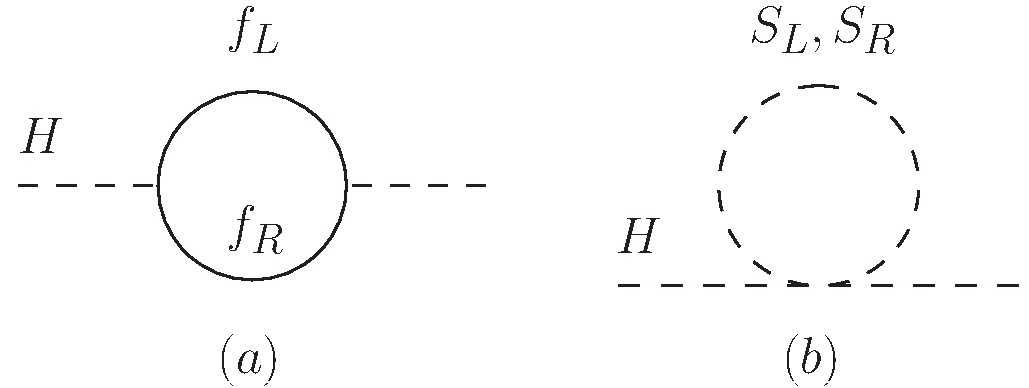
\includegraphics[width=0.6\hsize]{loop_correction.pdf}
  \caption{One-loop correction to the Higgs mass from (a) a Weyl fermion $f$ and (b) a complex scalar $S$.}
  \label{fig:loop_correction}
\end{figure}

The MSSM is the simple extension of the SM with $\mathcal{N} = 1$ supersymmetry (SUSY).\footnote
{
  For a brief review of the $\mathcal{N} = 1$ SUSY gauge theory, see Sec.~\ref{sec:susy}.
}
One of the motivations to introduce SUSY is to solve the so-called hierarchy (or naturalness) problem \cite{Weinberg:1975gm,Gildener:1976ai,Susskind:1978ms} in the SM.
The problem is related to the quantum correction to the SM Higgs boson mass from heavy new physics particles.
For example, we can consider the one-loop correction to the Higgs mass from a Weyl fermion $f$ and a complex scalar $S$, both of which couple to the Higgs, as illustrated in Fig.~\ref{fig:loop_correction}.
The corrections to the Higgs mass is given by
\begin{align}
  \Delta m_h^2 &= -\frac{|\lambda_f|^2}{8 \pi^2} \left[
  \Lambda_{\mathrm{UV}}^2 + \mathcal{O} (\log(\Lambda_{\mathrm{UV}})) \right] & &\mathrm{(fermion)}, \label{eq:delmh_f}\\
  \Delta m_h^2 &= \frac{\lambda_S}{16 \pi^2} \left[
  \Lambda_{\mathrm{UV}}^2 + \mathcal{O} (\log(\Lambda_{\mathrm{UV}})) \right] & &\mathrm{(scalar)}, \label{eq:delmh_S}
\end{align}
where $\lambda_f$ is the Higgs-fermion coupling constant, while $\lambda_S$ the same for the scalar $S$.
We take the cut-off scale of the theory to be $\Lambda_{\mathrm{UV}}$ to regularize the otherwise divergent loop integral and neglect the lower order terms of $\Lambda_{\mathrm{UV}}$.
Eqs.~\eqref{eq:delmh_f} and \eqref{eq:delmh_S} show the quadratic dependence of $\Delta m_H^2$ on $\Lambda_{\mathrm{UV}}$, which means that the Higgs mass is sensitive to the energy scale of the beyond the SM physics.
However, there is at least one extremely high energy scale physics in nature, gravity at the Planck scale $M_{\mathrm{pl}} \sim 10^{18 \hyphen 19}\,\mathrm{GeV}$.
By substituting $\Lambda_{\mathrm{UV}} = M_{\mathrm{pl}}$ in Eqs.~\eqref{eq:delmh_f} and \eqref{eq:delmh_S} and assuming $\lambda_f \sim \lambda_S \sim \mathcal{O} (1)$, we notice that orders-of-magnitude fine-tuning is required to obtain the correct Higgs mass $m_h = 125.10\,\mathrm{GeV}$ \cite{Tanabashi:2018oca}, which is unnatural.

SUSY provides a nice solution to this fine-tuning problem.
As is summarized in Appendix~\ref{sec:susy}, each Weyl fermion in a supersymmetric model is accompanied by two complex scalars with the same mass $m_f = m_S$.
In addition, their coupling constants to the Higgs boson should have a relationship $|\lambda_f|^2 = \lambda_S$ because $\lambda_S$ is a coupling constant in the F-term potential sourced by a superpotential term proportional to $\lambda_f$.
By using both equations and summing the corrections \eqref{eq:delmh_f} and \eqref{eq:delmh_S} with a factor of two multiplied to the latter, we obtain a result without the quadratic dependence on the cut-off scale $\Lambda_{\mathrm{UV}}$ without fine-tuning.
This cancellation is ensured by the so-called non-renormalization theorem. \cite{Salam:1974jj, Grisaru:1979wc}

\begin{table}[t]
  \centering
  \begin{tabular}{c|ccc|cc}
    Notation & $SU(3)_C$ & $SU(2)_L$ & $U(1)_Y$ & boson & fermion \\ \hline
    $\hat{Q}_i$ & $\bm{3}$ & $\bm{2}$ & $1/6$ & squark & left-handed quark \\
    $\hat{L}_i$ & $\bm{1}$ & $\bm{2}$ & $-1/2$ & slepton & left-handed lepton \\
    $\hat{U}_i$ & $\bar{\bm{3}}$ & $\bm{1}$ & $-2/3$ & squark & right-handed up-type quark \\
    $\hat{D}_i$ & $\bar{\bm{3}}$ & $\bm{1}$ & $1/3$ & squark & right-handed down-type quark \\
    $\hat{E}_i$ & $\bm{1}$ & $\bm{1}$ & $1$ & slepton & right-handed lepton\\
    $\hat{H}_u$ & $\bm{1}$ & $\bm{2}$ & $1/2$ & Higgs & Higgsino\\
    $\hat{H}_d$ & $\bm{1}$ & $\bm{2}$ & $-1/2$ & Higgs & Higgsino
  \end{tabular}
  \caption{
    Notations and quantum numbers of the chiral superfields in the MSSM.
    Also shown are names of bosonic and fermionic components of each superfield used in this thesis.
  }
  \label{tab:mssm_csf}
\end{table}

\begin{table}[t]
  \centering
  \begin{tabular}{c|ccc|cc}
    Notation & $SU(3)_C$ & $SU(2)_L$ & $U(1)_Y$ & boson & fermion \\ \hline
    $\hat{g}$ & $\bm{8}$ & $\bm{1}$ & $0$ & gluon & gluino \\
    $\hat{W}$ & $\bm{1}$ & $\bm{3}$ & $0$ & $W$ boson & Wino\\
    $\hat{B}$ & $\bm{1}$ & $\bm{1}$ & $0$ & $B$ boson & Bino\\
  \end{tabular}
  \caption{
    Notations and quantum numbers of the vector superfields in the MSSM.
    Also shown are names of bosonic and fermionic components of each superfield.}
  \label{tab:mssm_vsf}
\end{table}

We now summarize the notations and quantum numbers of the chiral and vector superfields in the MSSM in Table~\ref{tab:mssm_csf} and \ref{tab:mssm_vsf}, respectively.
In the tables, we also summarize the names of bosonic and fermionic components of each superfield used in this thesis.
The supersymmetric part of the MSSM Lagrangian is described by the superpotential\footnote
{
  For a more detailed review of the MSSM, see for example~\cite{Martin:1997ns}.
}
\begin{align}
  W = Y_u^{i j} \hat{U}_i \hat{Q}_j \hat{H}_u - Y_d^{i j} \hat{D}_i \hat{Q}_j \hat{H}_d
  - Y_e^{i j} \hat{E}_i \hat{L}_j \hat{H}_d + \mu \hat{H}_u \hat{H}_d,
  \label{eq:mssm_sup}
\end{align}
where $i,j=1,2,3$ label the quark and lepton generation, while $Q, L, U, D,$ and $E$ are superfields that contain the left-handed quark, left-handed lepton, right-handed up-type quark, right-handed down-type quark, and right-handed charged lepton, respectively.
In Eq.~\eqref{eq:mssm_sup}, proper contraction of $SU(3)_C$ and $SU(2)_L$ indices is assumed.
Note that two Higgs doublets $H_u$ and $H_d$ with opposite values of $U(1)_Y$ hypercharges are introduced, which is needed to cancel the contributions to the gauge anomaly from fermionic partners of the Higgs doublets.

Postulating SM gauge symmetries as a unique guideline to construct a model, there are a few more terms allowed in the superpotential:
\begin{align}
  W_{\Delta L=1} &= \lambda^{ijk} \hat{L}_i \hat{L}_j \hat{E}_k + \lambda^{'ijk} \hat{L}_i \hat{Q}_j \hat{D}_k
  + \mu^i \hat{L}_i \hat{H}_u, \label{eq:super_L} \\
  W_{\Delta B=1} &= \lambda^{''ijk} \hat{U}_i \hat{D}_j \hat{D}_k, \label{eq:super_B}
\end{align}
where $\Delta L=1$ and $\Delta B=1$ represents the breaking of the lepton and baryon numbers by one, respectively.
These terms with a lepton or baryon number breaking are phenomenologically problematic since they may cause a too fast proton decay, depending on parameters (see for example \cite{Sakai:1981pk}).
To avoid this problem, we often rely on a symmetry called the R-parity \cite{Farrar:1978xj} or the matter parity \cite{Dimopoulos:1981zb, Weinberg:1981wj, Sakai:1981pk, Dimopoulos:1981yj}.
Charges of the R-parity, which is basically a $Z_2$ symmetry, are calculated as
\begin{align}
  P_R = (-1)^{3(B-L)+2s},
\end{align}
where $B$, $L$, and $s$ are the baryon number, lepton number, and spin of the particle, respectively.
According to the definition, we can see that all the SM particles have even parity ($P_R = +1$), while all the supersymmetric particles have odd parity ($P_R = -1$).
Then it is easy to check that Eqs.\eqref{eq:super_L} and \eqref{eq:super_B} lead to the R-parity violating terms in the Lagrangian and thus are forbidden, while all the terms in Eq.~\eqref{eq:mssm_sup} are allowed.
From now on, we only focus on the R-parity preserving MSSM.

Since no superpartner of any SM particle is observed yet, SUSY should be broken at some scale to give large masses to superpartners.
The SUSY breaking part of the Lagrangian is expressed as
\begin{align}
  \mathcal{L}_{\mathrm{soft}} =&
  -\frac{1}{2} \left( M_3 \g \g + M_2 \W \W + M_1 \B \B + \mathrm{h.c.} \right) \notag \\&
  -\left( A_u^{ij} \U_i \Q_j H_u - A_d^{ij} \D_i \Q_j H_d - A_e^{ij} \E_i \L_j H_d \right) \notag \\&
  -m_Q^{2ij} \Q^\dagger_i \Q_j - m_L^{2ij} \L^\dagger_i \L_j - m_U^{2ij} \U^\dagger_i \U_j
  -m_D^{2ij} \D^\dagger_i \D_j - m_E^{2ij} \E^\dagger_i \E_j \notag \\&
  -m_{H_u}^2 H_u^{*} H_u - m_{H_d}^2 H_d^{*} H_d - \left( b H_u H_d + \mathrm{h.c.} \right),
  \label{eq:mssm_soft}
\end{align}
where the tilde is used to express the superpartner of the SM particle contained in a superfield, while fields without hat nor tilde denote particles in the SM.
An exception is two Higgs doublets, where $H_u$ and $H_d$ express the scalar components, while $\tilde{H}_u$ and $\tilde{H}_d$ express their superpartners called Higgsinos.
The SM-like Higgs doublet $H$ corresponds to a linear combination of $H_u$ and $H_d$, while the other combination becomes heavy.

It is known that, within the MSSM, almost all SUSY breaking mechanisms, such as the F-term (O$^{\mathrm{\prime}}$Raifeartaigh) \cite{ORaifeartaigh:1975nky} or D-term (Fayet-Iliopoulos) SUSY breaking \cite{Fayet:1974jb, Fayet:1974pd}, fail to generate masses of superpartners with remaining the SM gauge group in the low energy effective theory.
Thus, we need a so-called hidden sector in addition to the MSSM sector, in which SUSY is spontaneously broken.
For the MSSM sector to have Lagrangian terms \eqref{eq:mssm_soft}, we also need some mediation mechanism of the SUSY breaking.
The relative size of the SUSY breaking parameters in Eq.~\eqref{eq:mssm_soft} and thus the phenomenology of the model highly depends on the mediation mechanism.
Among many mediation mechanisms of SUSY breaking, the anomaly mediated SUSY breaking \cite{Giudice:1998xp, Randall:1998uk} leads to an interesting phenomenology with relatively light WIMPs, so it will be reviewed later.


\subsubsection*{Dark matter candidate in the MSSM}

There is another motivation to consider the R-parity preserving MSSM; it naturally contains the candidate for DM.
Since there is a sizable amount of DM in the current universe, a DM candidate should be stable or have a sufficiently long lifetime.
In many models, the stability of DM is ensured by imposing a symmetry and/or by kinematically forbidding the DM decay.
In the MSSM, the role of stabilizer can be played by the R-parity described above.
Recalling that all the SM (supersymmetric) particles have even (odd) parity, each interaction vertex in the MSSM Lagrangian should contain an even number of supersymmetric particles.
If we consider the lightest supersymmetric particle (LSP), such vertices can not construct the kinematically allowed LSP decay chain and, as a result, the LSP becomes a stable DM candidate.

The DM phenomenology, such as the production and annihilation of DM in the universe and processes that allow us to efficiently detect it, highly depends on which species of the supersymmetric particle becomes the LSP.
Hereafter, we only focus on the cases where one of the gauginos and Higgsinos becomes the LSP, whose motivations are described below.
Besides, all the LSP candidates described below (\textit{i.e.,} Wino and Higgsino) have non-zero electroweak charges and they can be viewed as examples of the WIMPs.


\subsubsection*{Higgs mass in the MSSM}

Under the spontaneously or softly broken SUSY, the quantum correction to the Higgs boson is modified from that in the SUSY limit.
One obvious consequence of the SUSY breaking is the hierarchy between the fermion and scalar masses that affects the logarithmic corrections to the Higgs mass.
In the case of the MSSM, the largest contribution comes from the superpartner of the top quark, stop, which has the largest Yukawa coupling with the Higgs boson.

\begin{table}[t]
  \centering
  \begin{tabular}{ccc}
    Value & Description & Reference\\ \hline
    $M_W = 80.384 \pm 0.014\, \mathrm{GeV}$ & Pole mass of the W boson
      & \cite{Group:2012gb,Alcaraz:1016509} \\
    $M_Z = 91.1876 \pm 0.0021\, \mathrm{GeV}$ & Pole mass of the Z boson
      & \cite{Beringer:1900zz} \\
    $M_h = 125.15 \pm 0.24\, \mathrm{GeV}$ & Pole mass of the Higgs
      & \cite{Aad:2013wqa,Chatrchyan:2013mxa} \\
    $M_t = 173.34 \pm 0.82\, \mathrm{GeV}$ & Pole mass of the top quark
      & \cite{ATLAS:2014wva} \\
    $\left( \sqrt{2} G_\mu \right)^{-1/2} = 246.21971 \pm 0.00006\, \mathrm{GeV}$
      & Fermi constant for $\mu$ decay & \cite{Tishchenko:2012ie} \\
    $\alpha_3 (M_Z) = 0.1184 \pm 0.0007$
      & $\overline{\mathrm{MS}}$ $SU(3)_C$ gauge coupling & \cite{Bethke:2012jm}
  \end{tabular}
  \caption{Experimentally measured SM parameters used for the derivation of Eq.~\eqref{eq:lambda_at_top}.}
  \label{tab:SM_param}
\end{table}

When there is a large hierarchy between the SUSY breaking scale $M_S$, which is comparable to stop masses, and the top mass $M_t$, the stop contributions to the Higgs mass contain a large logarithm of the form of $\log \left( M_S^2 / M_t^2 \right)$.
To resum the large logarithm and obtain a precise result, an easy way is to rely on the renormalization group equation (RGE).
In this framework, the value of the Higgs self-coupling $\lambda$ at the electroweak scale is closely related to the Higgs mass.
We define the potential for the SM Higgs doublet $H$ as
\begin{align}
  V(H) = -\frac{m^2}{2} |H|^2 + \lambda |H|^4,
\end{align}
and assume the SM parameters summarized in Table~\ref{tab:SM_param}.
Then, according to \cite{Buttazzo:2013uya}, we obtain the relationship\footnote
{
  Although the values listed in Table~\ref{tab:SM_param} are different from the latest ones given in \cite{Tanabashi:2018oca}, we use older ones because the change in input values may cause the slight change in values in Eq.~\eqref{eq:lambda_at_top}.
  The latest central values of the Higgs and top masses are $M_h = 125.10\,\mathrm{GeV}$ and $M_t = 173.1\,\mathrm{GeV}$, with which we can estimate $\lambda (M_t) = 0.12595$.
}
\begin{align}
  \lambda (M_t) = 0.12604
  + 0.00206 \left( \frac{M_h}{\mathrm{GeV}} - 125.15 \right)
  - 0.00004 \left( \frac{M_t}{\mathrm{GeV}} - 173.34 \right),
  \label{eq:lambda_at_top}
\end{align}
where the $\overline{\mathrm{MS}}$ scheme is used to renormalize the divergence of loop integrals.

In the MSSM, the value of $\lambda$ at the SUSY breaking scale $M_S$ is given by
\begin{align}
  \lambda (M_S) = \frac{g_1^2 (M_S) + g_2^2 (M_S)}{8} \cos^2 2\beta + \delta \lambda,
  \label{eq:lambda_at_ms}
\end{align}
where $g_1$ and $g_2$ are $U(1)_Y$ and $SU(2)_L$ gauge coupling constants, respectively, while $\beta$ parametrizes the ratio of the vacuum expectation values
\begin{align}
  \frac{\Braket{H_u^0}}{\Braket{H_d^0}} = \tan \beta,
\end{align}
with $H_u^0$ and $H_d^0$ being electromagnetically neutral components of the corresponding Higgs doublets.
In Eq.~\eqref{eq:lambda_at_ms}, the first term shows the tree-level contribution from the D-term potential and $\delta \lambda$ denotes the threshold correction from heavy superpartners.
$M_S$ is often chosen to be the geometric mean of stop masses to minimize the largest contribution to $\delta \lambda$ from stops.
Once the spectrum of the MSSM particles is fixed, we can evaluate the Higgs self-coupling using Eq.~\eqref{eq:lambda_at_ms}, calculate its running according to the RGE, and obtain the prediction for the Higgs mass through Eq.~\eqref{eq:lambda_at_top}.

\begin{figure}[t]
  \centering
  \includegraphics[width=0.6\hsize]{higgs_mass.pdf}
  \caption{
    Contour of the Higgs mass $m_h$ in the $\tan\beta$ vs. $M_S$ plane.
    The universal mass $M_S$ is assumed for all the SUSY particles.
    Blue (red) lines correspond from top to bottom to the contours of $m_h = 131, 128, 125, 122, 119\, \mathrm{GeV}$ for the minimal (maximal) stop mixing.
    Gray shade corresponds to the region where $m_h = 125.10\,\mathrm{GeV}$ can be explained.
  }
  \label{fig:higgs_mass}
\end{figure}

In Fig.~\ref{fig:higgs_mass}, we show the contour plot of the Higgs mass $m_h$ in the $\tan\beta$ vs. $M_S$ plane.
We assume the universal mass $M_S$ for all the SUSY particles and use the RGEs summarized in \cite{Buttazzo:2013uya}.
Under this assumption, the largest contribution to the threshold correction $\delta \lambda$ from stops is expressed as
\begin{align}
  \delta \lambda &\simeq \frac{9 y_t^2 (M_S)}{16 \pi^2} \tilde{X}_t \left[ 1-\frac{\tilde{X}_t}{12} \right], \label{eq:del_lambda}\\
  \tilde{X}_t &\equiv \frac{(A_t - \mu \cot \beta)^2}{M_S^2},
\end{align}
with $y_t \equiv Y_u^{33}$ and $A_t \equiv A_u^{33}$.
It is obvious from Eq.~\eqref{eq:del_lambda} that, for a moderate value of $\tilde{X}_t \lesssim 6$, $\tilde{X}_t = 0$ ($\tilde{X}_t = 6$) corresponds to the case with minimum (maximum) threshold correction, often called as the minimal (maximal) stop mixing.\footnote
{
  Eq.~\eqref{eq:del_lambda} shows that $\delta \lambda < 0$ for $\tilde{X}_t > 12$, resulting in the prediction of a lighter Higgs mass than the minimal stop mixing case.
  However, the parameter space with $\tilde{X}_t \gtrsim 6$ is severely constrained by the requirement of the stability of the electroweak vacuum (see for example \cite{Bagnaschi:2014rsa}) and is not considered here.
}

The red (blue) lines in Fig.~\ref{fig:higgs_mass} denote from top to bottom the contours of $m_h = 131$, $128$, $125$, $122$, and $119\, \mathrm{GeV}$ for the minimal (maximal) stop mixing.
Gray shade corresponds to the region where the central value of the observation $m_h = 125.10\,\mathrm{GeV}$ can be explained.
From the figure, we can see that the discovery of the Higgs with $m_h = 125.10\,\mathrm{GeV}$ may indicate a somewhat heavy SUSY breaking scale $M_S \gtrsim 10\,\mathrm{TeV}$ for the case with a small stop mixing or a small $\tan \beta$.
Combined with the fact that there is still no sign of the superpartners at the collider experiment, this motivates us to consider a heavy SUSY scenario.


\subsubsection*{Light Higgsino and its relation to the naturalness}

When we consider a heavy SUSY model concerning the Higgs mass, there is another problem called the little hierarchy problem.
This mentions the hierarchy between the electroweak scale and the heavy SUSY breaking scale and an accompanying fine-tuning.
Although the degree of the required fine-tuning is several orders of magnitude smaller than that for the large hierarchy between the electroweak and Planck scales, it will be more acceptable if some mechanism relieves the fine-tuning.
The required fine-tuning can be clearly expressed in the equation
\begin{align}
  \frac{1}{2} m_Z^2 = \frac{m_{H_d}^2 - m_{H_u}^2 \tan^2 \beta}{\tan \beta^2 - 1} - \mu^2,
\end{align}
where the right-handed side is the MSSM prediction for the $Z$-boson mass assuming the successful electroweak symmetry breaking.
If some of the MSSM parameters $m_{H_d}$, $m_{H_u}$, $\mu$ are much larger than $m_Z$, there should be some amount of fine-tuning to satisfy the equation.

There is a measure of the fine-tuning in this sense, proposed in \cite{Ellis:1986yg,Barbieri:1987fn}:
\begin{align}
  \Delta_{a_i} \equiv \frac{a_i}{m_Z^2} \frac{\partial m_Z^2}{\partial a_i},
\end{align}
where $a_i$ is an MSSM model parameter.
In order for the model to be ``natural'', we require $|\Delta_{a_i}| < \Delta$ for any $a_i$ with a typical choice of $\Delta \sim \mathcal{O}(10 \hyphen 100)$.
Since $m_Z$ is sensitive to the Higgsino mass $\mu$, this gives an upper bound on the ``natural'' choice of the Higgsino mass
\begin{align}
  \mu^2 < \frac{m_Z^2}{2} \Delta,
\end{align}
predicting the (sub-)TeV scale Higgsino.
As we will see in Sec.~\ref{sec:relic}, the light Higgsino is also fascinating as a dark matter candidate.

Even when the SUSY breaking scale is much higher than the electroweak scale, it is not strange for Higgsino to be around the electroweak scale since it is protected by an R-symmetry and a Peccei Quinn symmetry.
The symmetry protection is also important for a solution to the so-called ``$\mu$-problem'' \cite{Giudice:1988yz}, where the large hierarchy between the SUSY preserving parameter $\mu$ and the cut-off scale of the MSSM such as $M_{\mathrm{pl}}$ is discussed.
When we consider the low energy effective field theory in which SUSY is broken and all the squarks and sleptons are decoupled, a unique linear combination of the R-symmetry and the Peccei Quinn symmetry is enhanced only if both gauginos and Higgsinos are massless.
This fact leads to the framework of the split SUSY \cite{Giudice:2004tc}, in which there is a hierarchy between the masses of Higgsinos/gauginos and the other SUSY particles.
In this framework, the phenomenology is determined by the ordering and hierarchy of Higgsino and gaugino masses.
In particular, the collider phenomenology of Higgsino will be summarized in Sec.~\ref{sec:direct} for the case when gauginos are heavier than Higssino.

Finally, the naturalness requirement discussed above also imposes an upper bound on other parameters, in particular, on $m_{H_u}^2$ for $\tan^2 \beta \gg 1$.
The small value of $m_{H_u}^2$ can be realized by the focus point mechanism \cite{Feng:1999hg, Feng:1999mn, Feng:1999zg}, where the choice of the SM parameters in our universe, particularly that of $y_t$, allows $m_{H_u}^2$ at the low energy scale to be insensitive to its boundary condition at the high energy scale.


\subsubsection*{Light Wino in the anomaly mediated SUSY breaking model}

Among many heavy SUSY models, the pure gravity mediation scenario \cite{Ibe:2006de, Ibe:2011aa, ArkaniHamed:2012gw} based on the anomaly mediated SUSY breaking \cite{Giudice:1998xp, Randall:1998uk} is of particular interest since it naturally predicts the existence of WIMPs (in particular Winos) in the TeV range.
In this scenario, the SUSY breaking effect is directly mediated to the quark and lepton supermultiplets, and they obtain masses comparable to the scale of the SUSY breaking, which is roughly equal to the gravitino mass $m_{3/2}$.
Higgsino is also considered to be heavy contrary to the model described above.
In fact, it is easy to realize the hidden sector dynamics that generate the $\mu$-term of $\mathcal{O} (m_{3/2})$.
On the other hand, the superpartners of gauge bosons, gauginos, feel the SUSY breaking effect only through a one-loop diagram, which is related to the conformal anomaly.
As a result, gaugino mass parameters in Eq.~\eqref{eq:mssm_soft} are one-loop suppressed compared with other mass parameters and given by
\begin{align}
  M_i (M_S) = -\left. \frac{\beta_i}{2 g_i^2} \right|_{M_S} m_{3/2},
\end{align}
where $i=1,2,3$ is a gauge index and $\beta_i$ denote the beta functions of gauge coupling constants.
At the one-loop level, this gives
\begin{align}
  M_1 (M_S) &= \frac{11 g_1^2 (M_S)}{16 \pi^2} m_{3/2},\\
  M_2 (M_S) &= \frac{g_2^2 (M_S)}{16 \pi^2} m_{3/2},\\
  M_3 (M_S) &= -\frac{3 g_3^2 (M_S)}{16 \pi^2} m_{3/2}.
\end{align}

Since Higgsinos are assumed to have a mass comparable to $m_{3/2} \sim M_S$, they decouple from the effective theory below the scale $M_S$.
To take account of the correction to the gaugino masses from the Higgs-Higgsino loop, one has to include the threshold correction at $M_S$
\begin{align}
  \Delta M_1 = \frac{g_1^2 (M_S)}{16\pi^2} L,
  ~~
  \Delta M_2 = \frac{g_2^2 (M_S)}{16\pi^2} L,
\end{align}
with
\begin{align}
  L \equiv \mu \sin 2\beta \frac{m_A^2}{|\mu|^2 - m_A^2} \ln \frac{|\mu|^2}{m_A^2},
\end{align}
where $m_A$ is the mass of the heavy CP-odd Higgs.

\begin{figure}
  \centering
  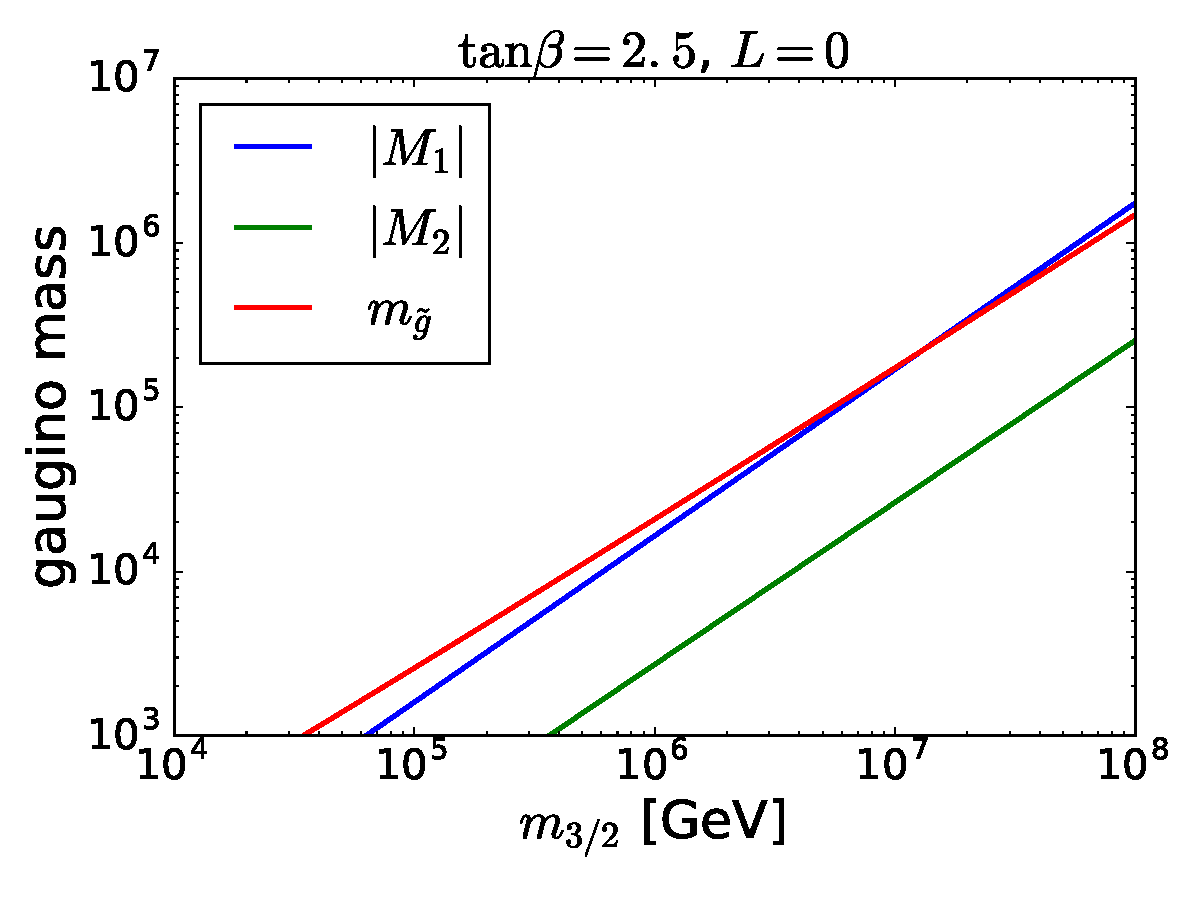
\includegraphics[width=0.48\hsize]{amsb_m32.pdf}
  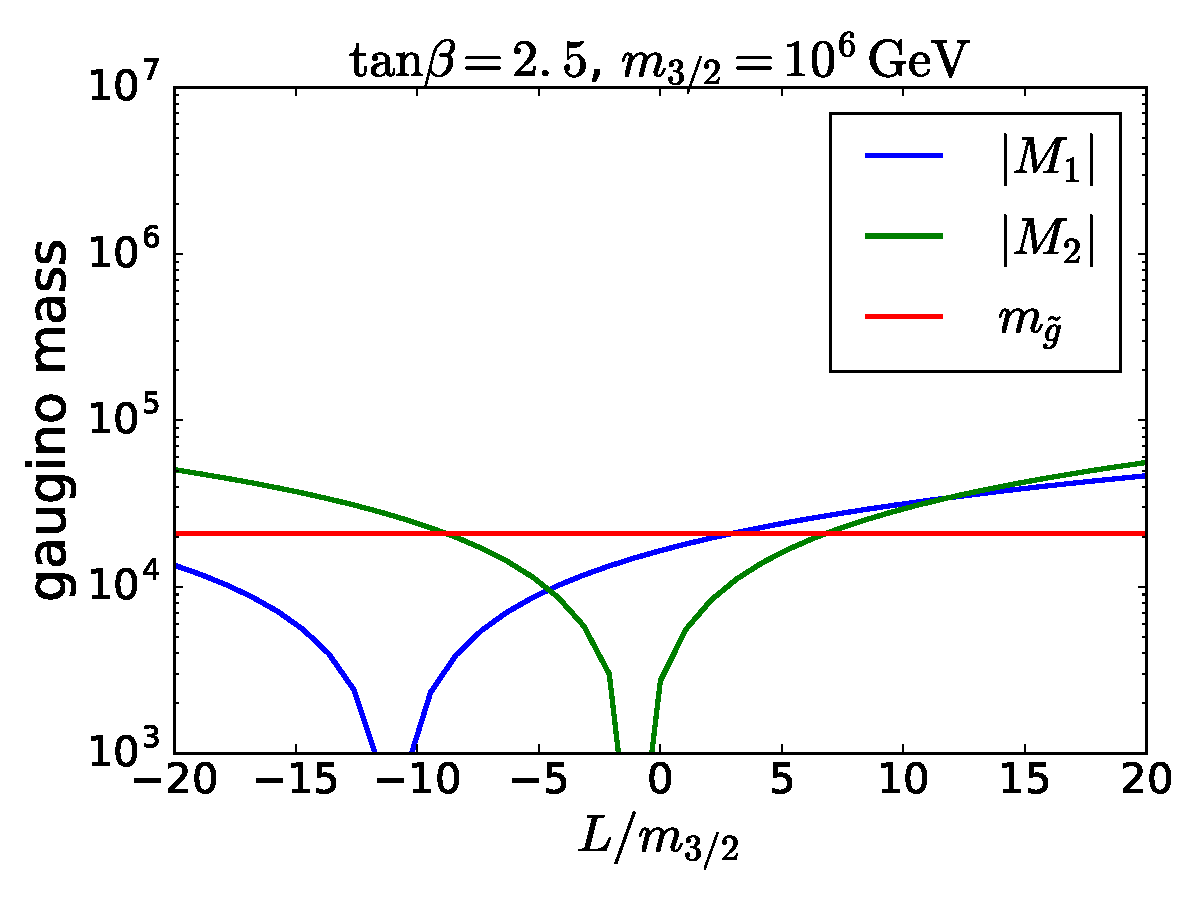
\includegraphics[width=0.48\hsize]{amsb_L.pdf}
  \caption{
    Gaugino masses as a function of $m_{3/2}$ with a fixed value of $L = 0$ (left) and that of $L / m_{3/2}$ with a fixed value of $m_{3/2} = 10^6\,\mathrm{GeV}$ (right).
    Blue, green, and red lines denote the masses of Bino, Wino, and gluino, respectively.
    $\tan\beta = 2.5$ is used in both figures.
  }
  \label{fig:amsb_spectrum}
\end{figure}

Below $M_S$, gaugino mass parameters further run towards the gaugino mass scale $M_{\tilde{G}}$, where the physical gaugino masses are determined.
Note that the Bino and Wino masses are well approximated by $|M_1 (M_{\tilde{G}})|$ and $|M_2 (M_{\tilde{G}})|$, while the gluino pole mass $m_{\tilde{g}}$ includes a sizable effect from the threshold correction as \cite{Giudice:2004tc}
\begin{align}
  m_{\tilde{g}} = \left| M_3 (M_{\tilde{G}}) \right| \left[
  1 + \frac{g_3^2}{16\pi^2} \left( 12 + 9\ln \frac{M_{\tilde{G}}^2}{|M_3|^2} \right)
  \right].
  \label{eq:mg_threshold}
\end{align}
The gaugino scale is often defined through $M_3 (M_{\tilde{G}}) = M_{\tilde{G}}$ to make the logarithmic term in Eq.~\eqref{eq:mg_threshold} vanish.

In Fig.~\ref{fig:amsb_spectrum}, we show the dependence of gaugino masses on $m_{3/2}$ and $L$.
In the left panel, we take $\tan\beta = 2.5$ and $L=0$, and the $m_{3/2}$ dependence is shown.
Blue, green, and red lines denote the masses of Bino, Wino, and gluino, respectively.
We can see that, throughout the parameter region used here, Wino becomes the lightest gaugino and becomes the LSP that can be a dark matter candidate.
In this choice of parameters, $m_{3/2} = 10^6\,\mathrm{GeV}$ roughly corresponds to the observed value of the Higgs mass $m_h \sim 125\,\mathrm{GeV}$, which at the same time realizes the $\mathcal{O}(1)\,\mathrm{TeV}$ mass for Wino.
As we will see in Sec.~\ref{sec:relic}, the Wino dark matter in this mass range is well-motivated since it gives us a collect relic abundance of the dark matter.

In the right panel of Fig.~\ref{fig:amsb_spectrum}, we also show the $L$ dependence of gaugino masses for $\tan\beta = 2.5$ and $m_{3/2} = 10^6\,\mathrm{GeV}$.
For simplicity, we neglect the relative phase of $m_{3/2}$ and $L$ and only consider the relative sign of them.
It can be seen that the hierarchy between gaugino masses is changed when a large value of $|L|$ is considered.
However, we can safely say that when the threshold correction is sufficiently small, $|L| \lesssim \mathcal{O}(m_{3/2})$, Wino remains to be the LSP.
Besides, the dependence of $m_h$ on $L$ is negligibly small and $m_h$ changes only $\mathcal{O} (0.1)\,\mathrm{GeV}$ within the parameter choice of the right panel.


%%%%%%%%%%%%%%%%%%%%%%%%%%%%%%%%%%%%%%%%%%%%%%%%%%%%%%%%%%%%%%%%%%%%%%%%%%%%%%%
\subsection{Minimal dark matter model}
\label{sec:MDM}
%%%%%%%%%%%%%%%%%%%%%%%%%%%%%%%%%%%%%%%%%%%%%%%%%%%%%%%%%%%%%%%%%%%%%%%%%%%%%%%

The MDM \cite{Cirelli:2005uq, Cirelli:2007xd, Cirelli:2009uv} is another example model that contains a WIMP DM candidate.
This model attempts to explain the existence of stable DM by extending the SM as simply as possible.
More specifically, we just assume the same gauge groups as the SM and add only one $SU(2)_L$ $n$-plet with $U(1)_Y$ hypercharge $Y$ in the model.\footnote
{
  This new particle, even if it is a fermion, does not contribute to the $SU(2)_L^2\, U(1)_Y$, $U(1)_Y^3$, nor $U(1)_Y\,\text{grav}^2$ anomalies when $Y=0$.
  When $Y \neq 0$, we always consider a vector-like pair of Weyl fermions, similar to the Higgsinos $\tilde{H}_u$ and $\tilde{H}_d$, which as a whole consists of a Dirac fermion and cancels the contributions to the gauge anomalies.
}

In some sense, WIMPs contained in the MSSM, if we assume all the other superpartners are decoupled, can also be viewed as an example of the MDM.
In fact, if we choose the set of $SU(2)_L$ and $U(1)_Y$ charges as $(n,Y) = (2,\pm 1/2)$ and $(3, 0)$, they correspond to the Higgsino and Wino, respectively.
However, for these choices, the stability of the $U(1)_{\mathrm{EM}}$ neutral component is not automatically ensured, and some extra symmetry (in this case the R-parity) is needed for the DM to survive until now.
The important point of the new framework MDM is that, when we use large $n \geq 5$, there are examples of multiplets that automatically contain a sufficiently long-lived DM candidate.

The stability of such multiplets can be understood through a simple group theoretical argument.
To write down the effective operator that describes the decay of an $n$-plet field to SM particles, we have to make an $n$-plet representation out of several SM fields.
However, since the largest $SU(2)_L$ representation in the SM is doublet, we need at least $n-1$ SM fields in the operator.
The operator made out of this large number of fields should be suppressed by a power of the cutoff scale $\Lambda$, at least by $\Lambda^{4-n}$ ($\Lambda^{3-n}$) for a scalar (fermion) MDM, and results in a small decay rate.
Since the well-motivated DM mass is of $\mathcal{O} (\mathrm{TeV})$ as we will see in Sec.~\ref{sec:relic}, the resulting lifetime of the DM candidate is estimated as $\tau \sim \Lambda^{-2p} (\mathrm{TeV})^{2p-1}$ for an operator with a suppression factor $\Lambda^{-p}$.
By demanding $\tau$ to be larger than the age of the universe under the assumption for the cut off scale $\Lambda < M_{\mathrm{pl}}$, we can conclude that the operator of the DM decay should have a dimension larger than five.
Then, we recast this condition to that for $n$ and obtain
\begin{align}
  n \geq
  \begin{cases}
    6 & \text{for scalar MDM},\\
    5 & \text{for fermion MDM}.
  \end{cases}
\end{align}

On the other hand, since we consider large $SU(2)_L$ multiplets, the RGE running of the $SU(2)_L$ gauge structure constant $\alpha_2$ above the MDM mass is drastically modified.
At the one-loop level, we have (see for example \cite{Machacek:1983tz})
\begin{align}
  \alpha_2^{-1} (Q) &= \alpha_2^{-1} (M_{\mathrm{MDM}}) - \frac{b_2}{2\pi} \ln \frac{Q}{M_{\mathrm{MDM}}},\\
  b_2 &\equiv -\frac{19}{6} + c\, \frac{n^3 - n}{18},
  \label{eq:b2_mdm}
\end{align}
with $c = 1$ $(1/4)$ for a Majorana/Weyl fermion (real scalar).
Note that the first and second terms of Eq.~\eqref{eq:b2_mdm} represent the contributions from SM particles and the MDM, respectively.
Then, assuming the perturbativity of the $SU(2)_L$ gauge coupling up to $M_{\mathrm{pl}}$, this relationship puts an upper bound on the choice of $n$.
According to the strong dependence on $n$ of $b_2$, a strong bound is obtained,
\begin{align}
  n \leq
  \begin{cases}
    8 & \text{real scalar MDM},\\
    5 & \text{Majorana fermion MDM}.
  \end{cases}
\end{align}

\begin{table}
  \centering
  \begin{tabular}{ccc|c|c|c}
    \multicolumn{3}{c|}{Quntum numbers} & DM & Not excluded by & Examples\\
    $SU(2)_L$ & $U(1)_Y$ & Spin & stability & direct detection & \\ \hline
    \hline
    2 & 1/2 & Scalar & & & \\
    2 & 1/2 & Fermion & & & Higgsino\\ \hline
    3 & 0 & Scalar & & $\checkmark$ & \cite{Farina:2013mla} \\
    3 & 0 & Fermion & & $\checkmark$ & Wino\\
    3 & 1 & Scalar/Fermion & & & \cite{Farina:2013mla} \\ \hline
    4 & 1/2 & Scalar/Fermion & & & \cite{Farina:2013mla} \\
    4 & 3/2 & Scalar/Fermion & & & \cite{Farina:2013mla} \\ \hline
    5 & 0 & Scalar & & $\checkmark$ & \cite{Farina:2013mla} \\
    5 & 0 & Fermion & $\checkmark$ & $\checkmark$ &
      \cite{Cirelli:2005uq, Cirelli:2007xd, Cirelli:2009uv} \\
    5 & 1 & Scalar & & & \\
    5 & 1 & Fermion & $\checkmark$ & & \\
    5 & 2 & Scalar & & & \\
    5 & 2 & Fermion & $\checkmark$ & & \\ \hline
    6 & 1/2, 3/2, 5/2 & Scalar & $\checkmark$ & & \\ \hline
    7 & 0 & Scalar & $\checkmark$ & $\checkmark$ &
      \cite{Cirelli:2005uq, Cirelli:2007xd, Cirelli:2009uv} \\
    7 & 1, 2, 3 & Scalar & $\checkmark$ & & \\
  \end{tabular}
  \caption{
    Table of the MDM properties.
    In the first three columns, we show the quantum numbers of our choice.
    In the next two columns, DM stability (the checkmark means ``stable'') and its status under the DM direct detection experiment (the checkmark means it is still alive) are shown.
    The last column is devoted to the examples in the literature.
  }
  \label{tab:mdms}
\end{table}

In Table~\ref{tab:mdms}, we summarize the properties of MDMs for several different choices of $(n, Y)$.
Throughout the table, the checkmark represents a suitable property as a DM candidate.
In the first three columns, we show the quantum numbers of our choice, namely the set of $(n,y)$ and spin.
In the next column, we show the condition for the DM stability, namely, whether all the DM decay operators have dimensions larger than five or not.
The checkmarks correspond to the automatically stable DM candidates.
The next column shows if the DM direct detection experiment has already excluded these DM candidates or not.
Since the non-zero value of $Y$ usually leads to the large cross section as will be discussed in Sec.~\ref{sec:direct_detection}, only $Y=0$ candidates are associated with checkmarks.
However, note that these properties may be changed due to a small modification to the model, such as the imposition of an extra symmetry or the mixing between other new physics particles.
The final column shows examples of the viable DM candidates analyzed in the literature.

From the table, we can see that there are two fascinating targets, $5$-plet fermion and $7$-plet scalar both of which have $Y=0$.
Among them, we neglect the latter possibility because it has been pointed out \cite{DiLuzio:2015oha, DelNobile:2015bqo} that a dimension five operator combined with a loop consisted of the $\mathrm{TeV}$ scale $7$-plet scalar induces a sizable decay rate for the $U(1)_{\mathrm{EM}}$ neutral component.
Instead, we will take a $5$-plet scalar with $Y=0$ just as a working example, assuming that its stability is ensured by some other mechanism.


%%%%%%%%%%%%%%%%%%%%%%%%%%%%%%%%%%%%%%%%%%%%%%%%%%%%%%%%%%%%%%%%%%%%%%%%%%%%%%%
\subsection{Mass splitting among an $SU(2)_L$ multiplet}
\label{sec:mass_splitting}
%%%%%%%%%%%%%%%%%%%%%%%%%%%%%%%%%%%%%%%%%%%%%%%%%%%%%%%%%%%%%%%%%%%%%%%%%%%%%%%

As a final remark in this section, we consider an important property of $SU(2)_L$ multiplets after the spontaneous breakdown of the electroweak symmetry: the mass splitting among the components of a multiplet.
This mass splitting, which we will call $\Delta m_\chi$, is typically much smaller compared with the WIMP mass $m_\chi$, but its value is phenomenologically important as we will see in later sections.

First, we start with the tree-level propagation of heavy particles, such as the SUSY particles other than the LSP, or other unknown particles.
After integrating out all the heavy particles other than the SM particles or the light WIMP, we may obtain operators of the form of $\mathcal{O} = M_{i j} \chi_i \chi_j$, where $\chi$ denotes the WIMP multiplet and $i$ is the $SU(2)_L$ index.
This operator causes the mass splitting only when $M_{i j}$ transforms non-trivially under the $SU(2)_L$ symmetry.
Then, we can explicitly construct the lowest dimensional operator among those relevant for the mass splitting.
For Higgsino,
\begin{align}
  \mathcal{O} = \frac{1}{\Lambda} (\bar{\chi} H^{*}) (H \chi),
  \label{eq:Higgsino_mass_splitting}
\end{align}
where $\chi = (\tilde{H}_u, -i \sigma_2 \tilde{H}_d^{*})^t$, $H$ is the SM Higgs doublet with $Y = 1/2$, $\Lambda$ is the cut-off scale of the effective theory, \textit{i.e.}, the typical mass scale of the relevant heavy particles, and the parenthesis denotes the $SU(2)_L$ invariant product of fundamental representations.
Similarly, for Wino, \cite{Gherghetta:1999sw}
\begin{align}
  \mathcal{O} = \frac{1}{\Lambda^3} (H^\dagger \sigma^a H) (H^\dagger \sigma^b H) \tilde{W}^a \tilde{W}^b,
  \label{eq:Wino_mass_splitting}
\end{align}
is the lowest dimensional operator that causes the mass splitting.
A simple implication of this observation is that, for multiplets with large $n$, there are suppression factors that keep the tree-level mass splitting small.
For Wino, the suppression is of $\mathcal{O} (M_W^4 / \Lambda^3)$, which yields a splitting smaller than $10\,\mathrm{MeV}$ for heavy particles with a few $\mathrm{TeV}$ masses.
For fermionic MDMs with $n \gtrsim 5$, a similarly small mass splitting at the tree-level is expected.\footnote
{
  For scalar MDMs, there is another renormalizable operator that generates a mass splitting
  \begin{align*}
    \mathcal{O} = - \lambda_H \left( \chi^{*} \sigma^a \chi \right) \left( H^\dagger \sigma^a H \right).
  \end{align*}
  Here, we just assume that $\lambda_H$ is sufficiently small and the discussion below is not affected by the above term.
}
This is the main reason why the loop correction plays a more important role in the mass splitting of Wino and MDMs.

The situation is different for Higgsino because of the much less drastic suppression factor of $\mathcal{O} (M_W^2 / \Lambda)$, which generates $\mathcal{O} (100)\,\mathrm{MeV}$ mass splitting for $\Lambda \lesssim \mathrm{10}\,\mathrm{TeV}$.\footnote
{
  For the order estimation of the mass splitting, we have taken account of the size of the coupling constants omitted in Eq.~\eqref{eq:Higgsino_mass_splitting}, using the rough estimation $g_1^2 \sim g_2^2 \sim \mathcal{O} (10^{-1})$.
}
In fact, in models like the split SUSY, the mixing between Higgsino and heavier gauginos can generate the large mass splitting among the Higgsino components.
As a result, neutral components that originally forms a Dirac fermion splits into two Majorana fermions with mass difference $\Delta m_0$, and the charged components also become heavier than the lighter neutral component by $\Delta m_\chi^{\mathrm{(tree)}}$.
According to \cite{Fukuda:2017jmk}, their approximate expressions are given by
\begin{align}
  \Delta m_0 &\simeq \frac{M_W^2}{g_2^2} \left( \frac{g_1^2}{M_1} + \frac{g_2^2}{M_2} \right),\\
  \Delta m_\chi^{\mathrm{(tree)}} &\simeq \frac{M_W^2}{2 g_2^2} \left[
  \left( \frac{g_1^2}{M_1} + \frac{g_2^2}{M_2} \right)
  + \mathrm{sgn} (\mu) \sin 2\beta \left( \frac{g_1^2}{M_1} - \frac{g_2^2}{M_2} \right) \right],
  \label{eq:Higgsino_delm_tree}
\end{align}
assuming the CP invariance for simplicity.
Note that the results agree with the previous order estimation with $\Lambda \sim M_1$, $M_2$.

Next, we consider the loop correction to the WIMP masses.
When the loop is composed of heavy particles, the effective operator that causes the mass splitting again becomes the same as above, which is now associated with a small loop factor.
Thus, the largest contribution comes from the gauge boson $\hyphen$ WIMP loop.
For the charged components of Higgsino, the one-loop result is known: \cite{Fukuda:2017jmk}
\begin{align}
  \Delta m_\chi^{\mathrm{(rad)}} \simeq \frac{1}{2} \alpha_2 M_Z \sin^2 \theta_W
  \left( 1 - \frac{3 M_Z}{2\pi m_\chi} \right)
  \sim 355\,\mathrm{MeV} \left( 1 - \frac{3 M_Z}{2\pi m_\chi} \right),
  \label{eq:Higgsino_delm_rad}
\end{align}
with $\theta_W$ being the Weinberg angle, which gives $\Delta m_\chi^{\mathrm{(rad)}} \simeq 341\,\mathrm{MeV}$ for the thermal Higgsino DM mass $m_\chi = 1.1\,\mathrm{TeV}$ described in Sec.~\ref{sec:relic}.
This loop-level contribution is important in the evaluation of $\Delta m_\chi = \Delta m_\chi^{\mathrm{(tree)}} + \Delta m_\chi^{\mathrm{(rad)}}$.
On the other hand, for Wino, we have the two-loop result \cite{Ibe:2012sx}
\newcommand{\logmchi}{\left( \log \frac{m_\chi}{\mathrm{GeV}} \right)}
\begin{align}
  \frac{\Delta m_\chi}{\mathrm{MeV}} =
  &-413.315 + 305.383 \logmchi - 60.8831 \logmchi^2 \notag \\
  &+ 5.41948 \logmchi^3 - 0.181509 \logmchi^4,
\end{align}
which exhibits $\Delta m_\chi \simeq 165\,\mathrm{MeV}$ for the thermal Wino DM mass $m_\chi = 2.9\,\mathrm{TeV}$.\footnote{
  The authors of \cite{Ibe:2012sx} have checked the validity of the fitting formula within the range $100\, \mathrm{GeV} < m_\chi < 4\,\mathrm{TeV}$.
  For $m_\chi > 4\,\mathrm{TeV}$, the mass splitting still remains to be the asymptotic value $\Delta m \simeq 165\,\mathrm{MeV}$.
}
For the MDM, there are neutral, singly charged, doubly charged, and so on, components.
Among them, the neutral and singly charged components have the smallest mass difference of $\Delta m_\chi \simeq 166\, \mathrm{MeV}$ \cite{Cirelli:2005uq}, which is the most important value for the phenomenology.


%%%%%%%%%%%%%%%%%%%%%%%%%%%%%%%%%%%%%%%%%%%%%%%%%%%%%%%%%%%%%%%%%%%%%%%%%%%%%%%
\subsection{Summary table}
\label{sec:model_summary}
%%%%%%%%%%%%%%%%%%%%%%%%%%%%%%%%%%%%%%%%%%%%%%%%%%%%%%%%%%%%%%%%%%%%%%%%%%%%%%%

\begin{table}[t]
  \centering
  \begin{tabular}{c|ccc|cc}
    & \multicolumn{3}{c|}{Quantum numbers} & \multicolumn{2}{c}{Masses}\\
    WIMP DM candidate & $SU(2)_L$ & $U(1)_Y$ & Spin & $m_\chi / \mathrm{TeV}$ &
    $\Delta m_\chi / \mathrm{MeV}$ \\
    \hline
    Higgsino & $2$ & $1/2$ & Dirac fermion & 1.1 & $341 + \Delta m_\chi^{\mathrm{(tree)}}$ \\
    Wino & $3$ & $0$ & Majorana fermion & 2.9 & 165 \\
    5-plet fermion & $5$ & $0$ & Majorana fermion & 10 & 166\\
    5-plet scalar & $5$ & $0$ & real scalar & 9.4 & 166
  \end{tabular}
  \caption{
    Table of properties of WIMPs discussed in this thesis.
    In the ``Quantum numbers'' block, the $SU(2)_L$ and $U(1)_Y$ charges and spin nature are shown.
    In the ``Masses'' block, the proper mass $m_\chi$ of the thermally produced DM and mass difference between the neutral and charged components $\Delta m_\chi$ of the multiplet are shown.
    See Sec.~\ref{sec:relic} for the descriptions and implications of $m_\chi$.
  }
  \label{tab:WIMP_property}
\end{table}

In Table~\ref{tab:WIMP_property}, we summarize the properties of WIMPs discussed in this thesis.
In the first block named ``Quantum numbers'', we show the $SU(2)_L$ electroweak charge, $U(1)_Y$ hypercharge, and spin nature.
In the second block named ``Masses'', two types of masses are shown.
$m_\chi$ is the required masses to explain the DM relic abundance without non-thermal production (see Sec.~\ref{sec:relic} for the detail).
$\Delta m_\chi$ is the mass difference between the electromagnetically neutral and (singly) charged components of the multiplet discussed in the previous section.
Values are taken from \cite{Farina:2013mla, ArkaniHamed:2006mb, Hisano:2006nn,  Cirelli:2007xd, Moroi:2013sla, Beneke:2016ync}.

% \bibliographystyle{elsarticle-num}
% \bibliography{../phd}

\end{document}
